% Recognition-verified normalization pipeline (vector replacement for the
% legacy raster docs/normalise.png, which has no editable source).
%
% Content taken from normalization/verified.py and normalization/pipeline.py:
%   probe model      : weights/PP-OCRv6_det_small.onnx      (verified.py:32)
%   probe resolution : 640 px longer side                   (verified.py:33)
%   accept rule      : score_after >= 1.02 * score_before   (verified.py:38,151)
%   guards           : min(H,W) < 450 px; score_before <= 0 (verified.py:48,123,130)
%   forced order     : white balance -> rectify -> glare -> shadow -> CLAHE(std<45)
%
% Designed at ~7.2 in wide so it needs no downscaling at \textwidth in a
% two-column layout: the type sizes below are the ones that reach the page.
%
% Build:  pdflatex normalisation_verified.tex
\documentclass[border=5pt]{standalone}
\usepackage[T1]{fontenc}
\usepackage{times}
\usepackage{amsmath}
\usepackage{tikz}
\usetikzlibrary{arrows.meta, positioning, fit, backgrounds, calc}

\begin{document}
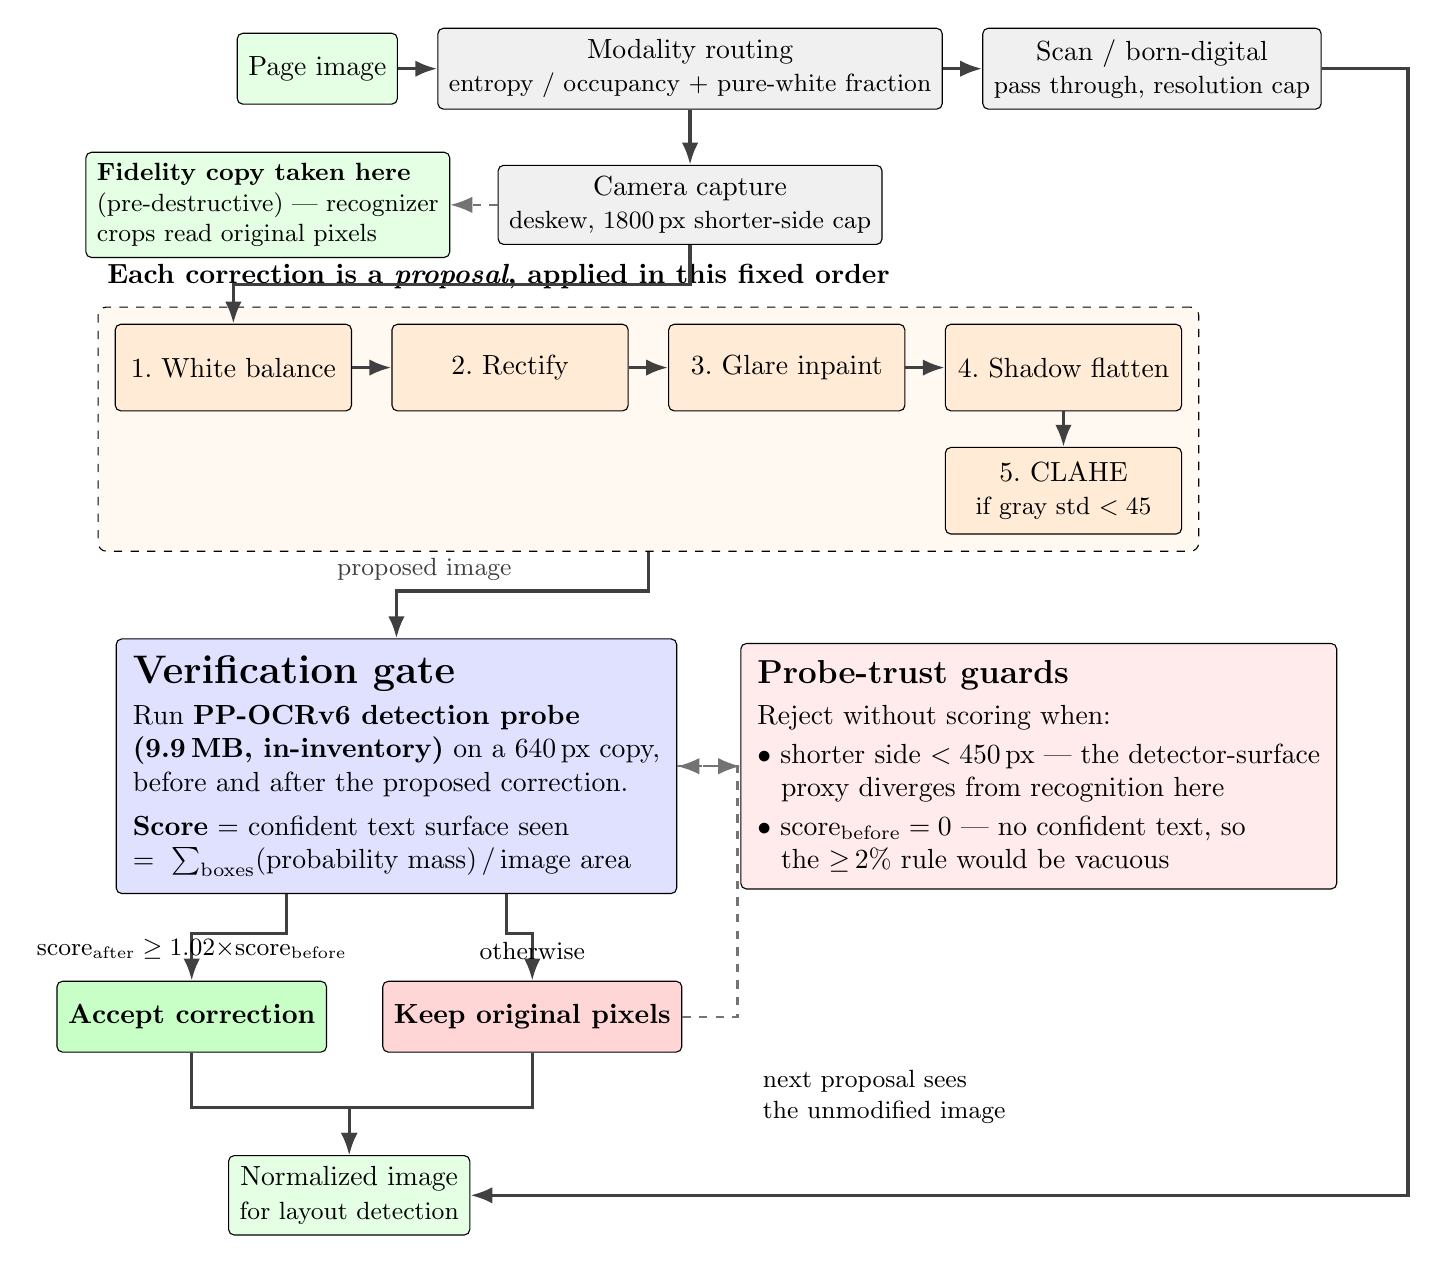
\begin{tikzpicture}[
  font=\normalsize,
  node distance=4.5mm and 5mm,
  box/.style   ={draw, rounded corners=2pt, align=center, inner sep=4pt,
                 minimum height=9mm, font=\normalsize},
  io/.style    ={box, fill=green!10},
  route/.style ={box, fill=gray!12},
  prop/.style  ={box, fill=orange!16, minimum width=30mm, minimum height=11mm},
  gate/.style  ={box, fill=blue!12, align=left, inner sep=6pt},
  acc/.style   ={box, fill=green!22, font=\normalsize\bfseries, minimum width=34mm},
  rej/.style   ={box, fill=red!16,   font=\normalsize\bfseries, minimum width=34mm},
  guard/.style ={box, fill=red!8, align=left, inner sep=6pt},
  arr/.style   ={-{Latex[length=2.8mm]}, very thick, black!75},
  darr/.style  ={-{Latex[length=2.8mm]}, thick, black!55, dashed},
]

% ================= row 1: input + modality routing =================
\node[io] (img) {Page image};
\node[route, right=of img] (mod)
  {Modality routing\\{\small entropy / occupancy + pure-white fraction}};
\node[route, right=of mod] (scan)
  {Scan / born-digital\\{\small pass through, resolution cap}};

\draw[arr] (img) -- (mod);
\draw[arr] (mod) -- (scan);

\node[route, below=7mm of mod] (cam)
  {Camera capture\\{\small deskew, 1800\,px shorter-side cap}};
\draw[arr] (mod) -- (cam);

% fidelity copy is taken here, before any destructive correction
\node[io, left=6mm of cam.west, anchor=east, align=left, font=\small] (fid)
  {\textbf{Fidelity copy taken here}\\(pre-destructive) --- recognizer\\crops read original pixels};
\draw[darr] (cam.west) -- (fid.east);

% ================= row 2: the proposal chain =================
\node[prop, below=10mm of cam.south, anchor=north, xshift=-58mm] (p1)
  {1.~White balance};
\node[prop, right=of p1] (p2) {2.~Rectify};
\node[prop, right=of p2] (p3) {3.~Glare inpaint};
\node[prop, right=of p3] (p4) {4.~Shadow flatten};

\node[prop, below=4.5mm of p4] (p5) {5.~CLAHE\\{\small if gray std $<45$}};

\begin{scope}[on background layer]
  \node[draw, dashed, rounded corners=3pt, fill=orange!5,
        fit=(p1)(p4)(p5), inner sep=6pt] (chain) {};
\end{scope}
\node[anchor=north west, font=\normalsize\bfseries, align=left]
  at ($(chain.north west)+(1.5mm,-1.5mm)$) {};
\node[anchor=south west, font=\normalsize\bfseries]
  at ($(chain.north west)+(0mm,1mm)$)
  {Each correction is a \emph{proposal}, applied in this fixed order};

\draw[arr] (cam.south) -- ++(0,-5mm) -| (p1.north);
\foreach \a/\b in {p1/p2, p2/p3, p3/p4}{\draw[arr] (\a) -- (\b);}
\draw[arr] (p4) -- (p5);

% ================= row 3: verification gate + guards =================
\node[gate, below=11mm of chain.south, anchor=north, xshift=-32mm] (gate) {%
  \textbf{\Large Verification gate}\\[3pt]
  Run \textbf{PP-OCRv6 detection probe}\\
  \textbf{(9.9\,MB, in-inventory)} on a 640\,px copy,\\
  before and after the proposed correction.\\[4pt]
  \textbf{Score} $=$ confident text surface seen\\
  $=\ \sum_{\text{boxes}}$(probability mass)\,$/$\,image area
};

\node[guard, right=8mm of gate.east, anchor=west] (guards) {%
  \textbf{\large Probe-trust guards}\\[3pt]
  Reject without scoring when:\\[2pt]
  $\bullet$~shorter side $<450$\,px --- the detector-surface\\
  \hspace*{3mm}proxy diverges from recognition here\\[2pt]
  $\bullet$~score$_{\text{before}}=0$ --- no confident text, so\\
  \hspace*{3mm}the $\geq$\,2\% rule would be vacuous
};

\draw[arr] (chain.south) -- ++(0,-5mm) -| node[above left, font=\small, pos=0.25]
  {proposed image} (gate.north);
\draw[darr] (gate.east) -- (guards.west);

% ================= row 4: decision + outputs =================
\node[acc, below=11mm of gate.south, anchor=north, xshift=-26mm] (accept)
  {Accept correction};
\node[rej, right=7mm of accept.east, anchor=west] (reject)
  {Keep original pixels};

\draw[arr] ($(gate.south)+(-14mm,0)$) -- ++(0,-5mm) -| (accept.north);
\node[font=\small, anchor=south, align=center] at ($(accept.north)+(0,1.5mm)$)
  {score$_{\text{after}}\geq 1.02\times$score$_{\text{before}}$};
\draw[arr] ($(gate.south)+(14mm,0)$) -- ++(0,-5mm) -| (reject.north);
\node[font=\small, anchor=south] at ($(reject.north)+(0,1.5mm)$) {otherwise};

% rejected proposal: the chain continues from the unmodified image
\draw[darr] (reject.east) -- ++(7mm,0) |- (gate.east);
\node[font=\small, align=left, anchor=north west]
  at ($(reject.south east)+(9mm,-1mm)$)
  {next proposal sees\\the unmodified image};

\node[io, below=13mm of accept.south, anchor=north, xshift=20mm] (out)
  {Normalized image\\{\small for layout detection}};
\draw[arr] (accept.south) -- ++(0,-7mm) -| (out.north);
\draw[arr] (reject.south) -- ++(0,-7mm) -| (out.north);

% scan / born-digital branch bypasses the whole gate, down the right margin
\coordinate (rt) at ($(guards.east)+(9mm,0)$);
\draw[arr] (scan.east) -- ++(6mm,0) -- (scan.east -| rt) -- (out.east -| rt)
  -- node[above, font=\small, pos=0.35] {} (out.east);

\end{tikzpicture}
\end{document}
